\section{The Usual, Spherical \Luscher's Formula}\label{sec:spherical}


Here we present a $D$-dimensional derivation of \Luscher's formula that roughly follows \Ref{Beane:2003da}, although the technology and sophistication of the finite-volume formalism has grown substantially \todo{cite cite cite}.  Assuming an interaction given by an tower of derivative contact operators
\begin{equation}
    V(p) = +\sum_n C_{2n}(\Lambda) p^{2n}
\end{equation}
where the interaction strengths depend on the regulator and carry spatial-dimension-dependent units.
The scattering amplitude is given by the bubble sum depicted in \Figref{bubbleSum}.

\begin{figure}[ht!]
\center
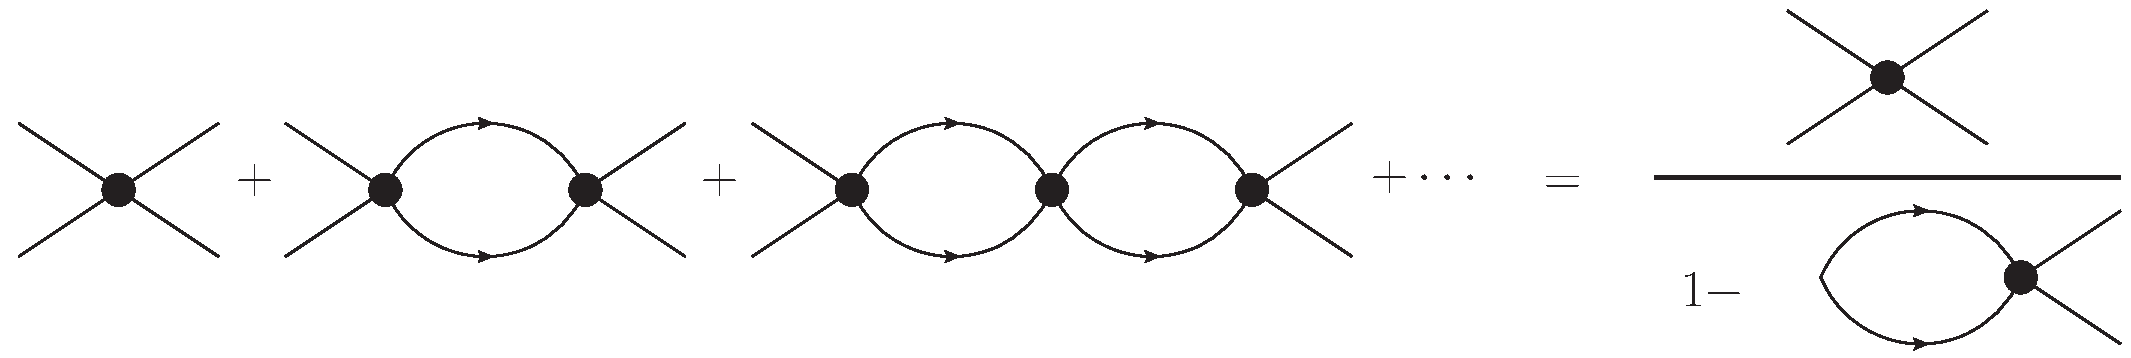
\includegraphics[width=\columnwidth]{figure/bubbleSum.pdf}
\caption{Bubble sum. Each line represents a propagator, each vertex represents $-i \sum_n C_{2n}(\Lambda) p^{2n}$, and the bubble is given by $I_0$ (see also \Figref{I0}).\label{fig:bubbleSum}}
\end{figure}

This bubble sum is a geometric series and gives, for the standard $T$-matrix, \cite{Kaplan:1998we,Beane:2003da}
\begin{equation}\label{eq:T matrix}
iT = \frac{-i\sum_n C_{2n}(\Lambda) p^{2n}}{1-I_0(p,\Lambda) \sum_n C_{2n}(\Lambda) p^{2n}},
\end{equation}
where $p$ is the relative momentum,  and $I_0(p,\Lambda)$ is a $D$-dependent function that arises from integrating the loop shown in \Figref{I0},
\begin{align}
    I_0(p)
    &=-i\int^{\Lambda}
        \frac { \mathrm {d}q_0}{2\pi}\ \frac{\mathrm { d } ^ { D } \vec{ q } } { (2\pi)^ { D } }
        \left( \frac { i } { \frac{E}{2} + q _ { 0 } - \frac{\vec{q}^2}{2m} + i \epsilon } \right)
        \left( \frac { i } { \frac{E}{2} - q _ { 0 } - \frac{\vec{q}^2}{2m} + i \epsilon } \right)
    \nonumber\\
    &=\frac{\Omega_D}{(2\pi)^D}\int^{\Lambda}  \mathrm { d } q \ q^{D-1}\left[\mathcal{P} \left( \frac { 1 } { E - \frac{\vec{q}^2}{m} } \right)
-i\frac{\pi m}{2q}\delta(q-\sqrt{mE})\right]
    \\
    &=\frac{\Omega_D}{(2\pi)^2}\frac{m}{L^{D-2}}\int^{\Lambda L/2\pi}  \mathrm { d } n \ n^{D-1}\left[\mathcal{P} \left( \frac { 1 } { \left(\frac{pL}{2\pi}\right)^2 - n^2 } \right)
-i\frac{\pi^2}{L n}\delta\left(\frac{2\pi}{L}n -p\right)\right]
    \label{eq:I0}
\end{align}
where $\mathcal{P}$ refers to Principle (Cauchy) Value, we have used the on-shell condition $mE=p^2$, and the geometric factor
\begin{equation}
\Omega_D=\frac{2\pi^{D/2}}{\Gamma(D/2)}=
    \begin{cases}
        4\pi    &   (D=3)\\
        2\pi    &   (D=2)\\
        2       &   (D=1)
    \end{cases}\ ,
\end{equation}

\begin{figure}[h!]
    \center
    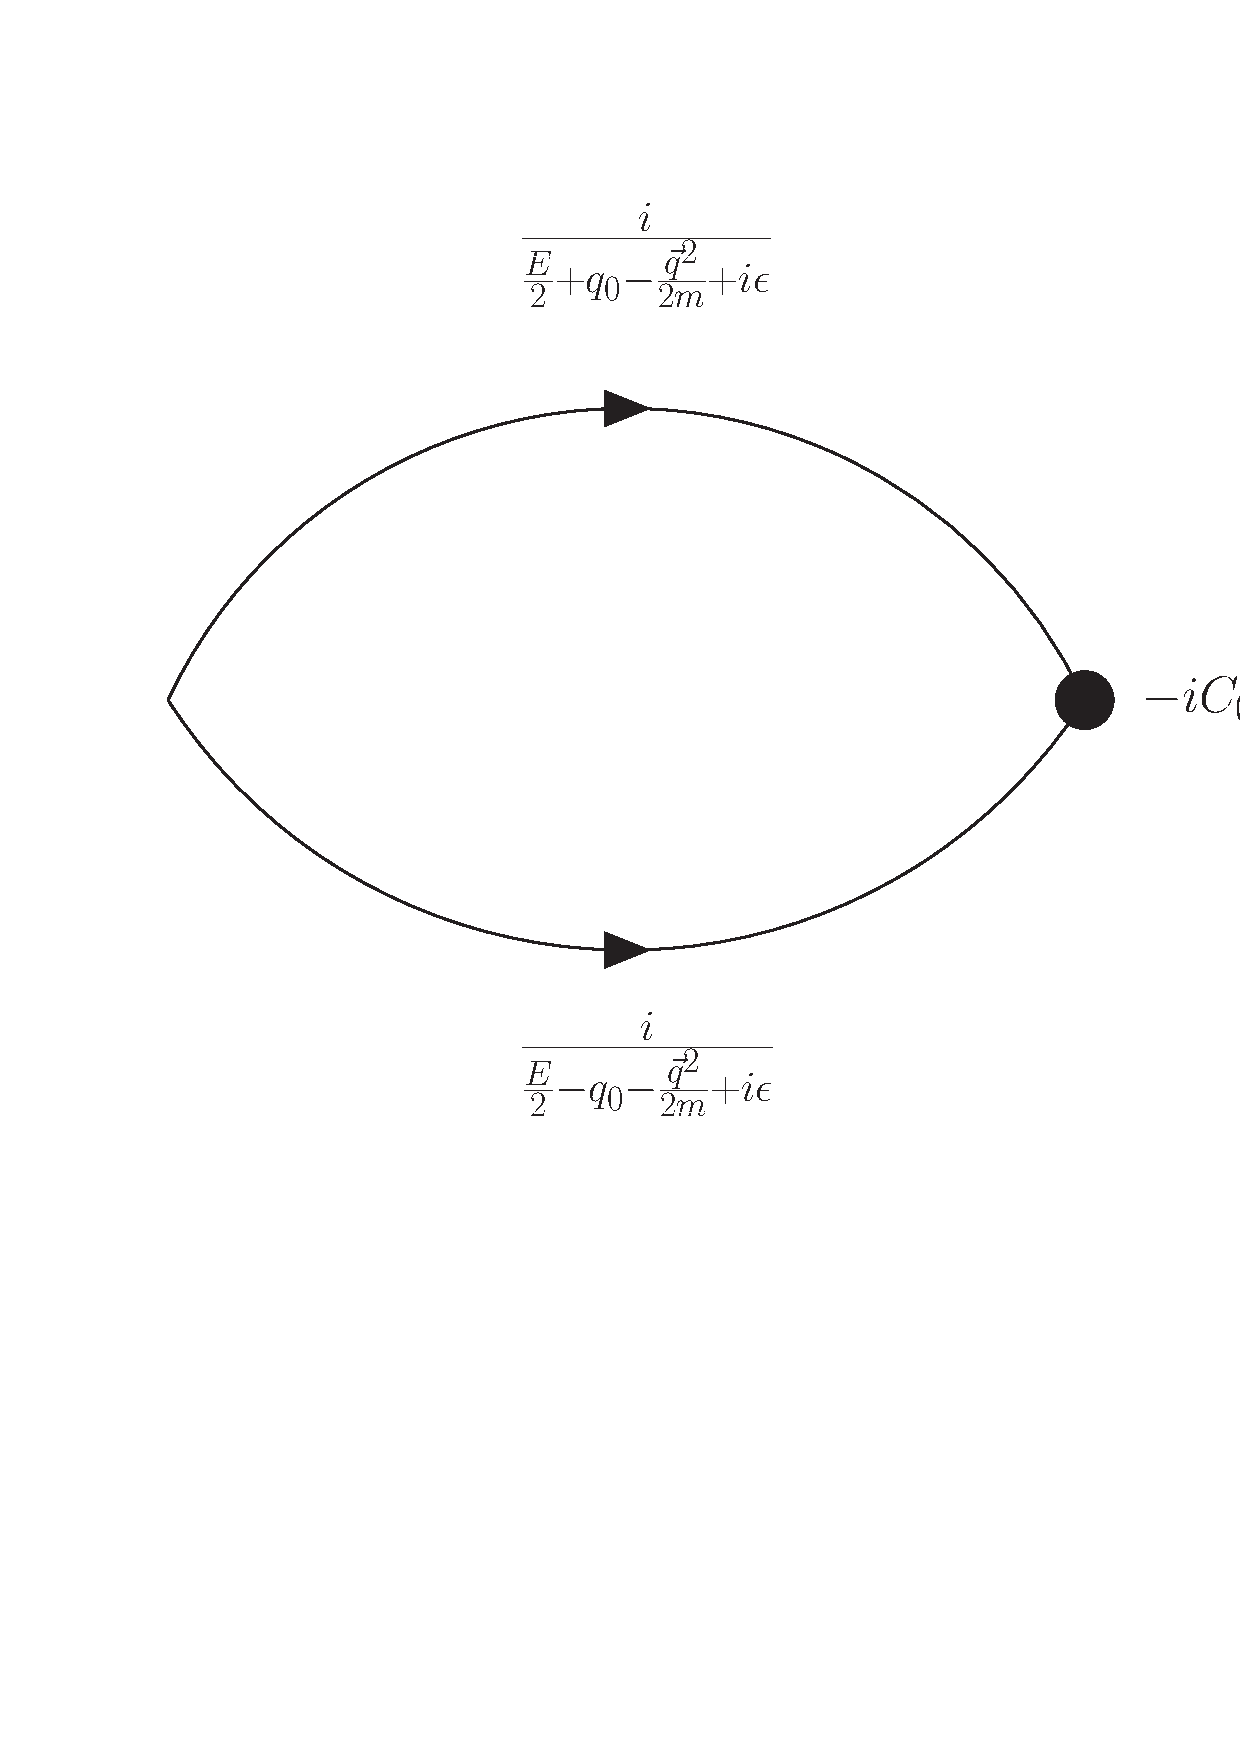
\includegraphics[width=.5\columnwidth]{figure/I0.pdf}
    \caption{
        Loop diagram contributing to the bubble sum.
        Because the potential is separable it factors out of the integral and $I_0$ is simply given by the loop of the two propagators.
    }
    \label{fig:I0}
\end{figure}

In the $s$-wave, the momentum-dependent $T$-matrix is related to the phase shift $\delta_0(p)$ by
\begin{equation}\label{eq:cot delta}
    i T = \frac{4}{m}\F_d\frac{i}{\cot \delta_0(p)-i}\ ,
\end{equation}
where
\begin{equation}
    \F_D
    =
    \begin{cases}
        \pi/p   & (D=3)\\
        1       & (D=2)\\
        p/2     & (D=1)
\end{cases}
\end{equation}
is a dimension-dependent kinematic factor.
This fixes the coefficients $C(\Lambda)$ as a function of the scattering data,
\begin{equation}\label{eq:IV pole}
    \frac{1}{\sum_n C_{2n}(\Lambda) p^{2n}}
    =
    I_0(p) - \frac{m}{4 \F_D}\left(\cot \delta_0(p) - i\right)
\end{equation}

In a finite volume, the energy eigenstates appear at poles of the $T$-matrix, so that
\begin{equation}\label{eq:FV pole}
    \frac{1}{\sum_n C_{2n}(\Lambda) p^{2n}} - I_{0,\FV}(p,L) = 0
\end{equation}
and the infinite-volume integral $I_0$ has been replaced by the matching finite-volume sum,
\begin{align}
I_{0,\FV}(p,L)
    &=-i\int \frac { \mathrm {d}q_0}{2\pi} \frac{1}{L^D}\sum_{\vec{q}}^{q < \Lambda} \left( \frac { i } { \frac{E}{2} + q _ { 0 } - \frac{\vec{q}^2}{2m} + i \epsilon } \right) \left( \frac { i } { \frac{E}{2} - q _ { 0 } - \frac{\vec{q}^2}{2m} + i \epsilon } \right)
    \\
    &=\frac{1}{L^D}\sum_{\vec{q}}^{q < \Lambda} \frac { 1 } { E - \frac{\vec{q}^2}{m} }
    =\frac{m}{(2\pi)^2 L^{D-2}} \sum_{\vec{n}}^{n < \frac{\Lambda L}{2\pi}} \frac{1}{x-n^2}
    &
    x &= \left( \frac{pL}{2\pi}\right)^2
\end{align}
where we have used the on-shell condition $mE=p^2$\todo{Be very careful about whether m is the reduced mass or not.}.  Combining the infinite-volume and finite-volume relations \eqref{IV pole} and \eqref{FV pole} yields
\begin{equation}
    \frac{m}{4\F_D}(\cot\delta_0(p)-i) = I_0(p) - I_{0,\FV}(p),
\end{equation}
the finite-volume quantization condition.

Plugging our results for the integrals in, one finds
\begin{equation}
    \frac{1}{4\F_D}\left(\cot \delta_0(p) - i\right) = \frac{1}{(2\pi)^2 L^{D-2}}\left[ \left(\int_{\vec{n}} - \sum_{\vec{n}}\right) \frac{1}{x-n^2} + \frac{-i \pi^2\Omega_D}{L} \int \mathrm{d}n\ n^{D-2} \delta\left(\frac{2\pi}{L}n - p\right) \right]
\end{equation}
where both the sum and integral are cut off by a restriction on the magnitude of $n$, $n^2 < (\Lambda L / 2\pi)^2$, and the integral implicitly carries a factor of $\Omega_D n^{D-1}$.
In a seemingly miraculous (but required) cancellation, the imaginary part on the left hand side exactly cancels the last term in the sum on the right, and we are left with
\begin{equation}
    \cot \delta_0(p) = \frac{\F_D}{\pi^2 L^{D-2}} \left(\sum_{\vec{n}}-\int_{\vec{n}}\right) \frac{1}{n^2-x}
\end{equation}
where $x=(pL/2\pi)^2$ and we switched the sign of the sum and integral as well as the sign of the denominator.
Because we cut off the sum and the integral in exactly the same way, in dimensions where $I_0$ diverges with $\Lambda$, the divergence cancels against the divergence in the sum.
Let $N=\Lambda L/2\pi$.
Then, defining, with a finite cutoff on magnitude $N/2$,
\begin{equation}\label{eq:spherical cutoff S}
    S^{\spherical N}_D(x) = \left(\sum_{\vec{n}}- \int_{\vec{n}}\right) \frac{1}{x-n^2}
\end{equation}
where the $\spherical$ superscript reminds us that we cut off our sum and integral in a spherical way, based on the magnitude of $n<N/2$, we recover the usual \Luscher zeta functions by taking
\begin{equation}\label{eq:spherical S}
    S^\spherical_D(x)
    =
    \lim_{N\goesto\infty} S^{\spherical N}_D(x)
    =
    \lim_{N\rightarrow\infty}\left( \sum_{\vec{n}}^{n < N/2} \frac{1}{x-n^2} - \counterterm_D^\spherical \left(\frac{N}{2}\right)^{D-2}\right)
\end{equation}
where dimension-dependent counterterm $\counterterm_D^\spherical$ comes from the integral; we evaluate said counterterms in \Appref{counterterm/spherical}.
Finally,
\begin{equation}\label{eq:spherical quantization}
    \cot \delta_0(p) = \frac{\F_D}{\pi^2 L^{D-2}} S^\spherical_D(x).
\end{equation}
This is the usual \Luscher finite-volume quantization condition, and continuum-extrapolated energy levels should be fed through it to produce continuum-limit scattering data.
In three dimensions it is common to move the momentum dependence in $\F_D$ to the other size, as $p \cot\delta_0(p)$ is what appears in the effective range expansion, as we will discuss in \Secref{ere}.

\todo{STILL REMAINING:}
\begin{itemize}
    \item ERE / matching
    \item Describe tuning
    \item Show results in 2, 3D
    \item Something is wrong :(?  More like :D because we are smart!
\end{itemize}
